\documentclass{article}

% if you need to pass options to natbib, use, e.g.:
% \PassOptionsToPackage{numbers, compress}{natbib}
% before loading nips_2016
%
% to avoid loading the natbib package, add option nonatbib:
%\usepackage[nonatbib]{nips_2016}

\usepackage{nips_2016}

% to compile a camera-ready version, add the [final] option, e.g.:
%\usepackage[final]{nips_2016}

\usepackage[utf8]{inputenc} % allow utf-8 input
\usepackage[T1]{fontenc}    % use 8-bit T1 fonts
\usepackage{hyperref}       % hyperlinks
\usepackage{url}            % simple URL typesetting
\usepackage{booktabs}       % professional-quality tables
\usepackage{amsfonts}       % blackboard math symbols
\usepackage{nicefrac}       % compact symbols for 1/2, etc.
\usepackage{microtype}      % microtypography
\usepackage{graphicx,psfrag,epsf,subcaption}
\usepackage[export]{adjustbox}
\usepackage{authblk}
\captionsetup[subfigure]{labelformat = empty,position=top}
\renewcommand{\bibsection}{}

\title{Matrix Explorer: A Web Application for Data Exploration}

% The \author macro works with any number of authors. There are two
% commands used to separate the names and addresses of multiple
% authors: \And and \AND.
%
% Using \And between authors leaves it to LaTeX to determine where to
% break the lines. Using \AND forces a line break at that point. So,
% if LaTeX puts 3 of 4 authors names on the first line, and the last
% on the second line, try using \AND instead of \And before the third
% author name.

\author{
  Ivan A. Kuznetsov \\
  Department of Bioengineering \\
  The Johns Hopkins University\\
  Baltimore, MD 21218 \\
  \texttt{ikuznet1@jhu.edu} \\
  \and
  Joshua T. Vogelstein \\
  Department of Bioengineering \\
  The Johns Hopkins University \\
  Baltimore, MD 21218 \\
  Institute for Computational Medicine \\
  The Johns Hopkins University \\
  Baltimore, MD 21218 \\
  \texttt{jovo@jhu.edu}
}

\begin{document}
% \nipsfinalcopy is no longer used

\maketitle

\begin{abstract}
  Exploration and visualization of tabular data is crucial to driving discovery across a multitude of different basic science fields. Unfortunately, given the vast array of various statistical tools that have been developed, finding the proper techniques to explore a novel dataset is more of an art than an exact science. Hence, researchers often choose the wrong tools to explore their data, leading to poor analysis. In this paper we describe Matrix Explorer, a novel data exploration and visualization web application that allows users to analyze uploaded tabular datasets. Within Matrix Explorer we have implemented techniques we believe are relevant to and best practice for any sorts of data analysis, including data visualization via heatmaps, scatter/line plots, marginal distributions, and two-dimensional embedding and data exploration via k-means clustering, dendrograms, correlation matrix computation, and outlier detection. We validated Matrix Explorer by showing that it produces correct results for the iris flower dataset.
\end{abstract}

\section{Introduction}
\label{sec:intro}

The past decade has seen an explosion in studies generating huge quantities of data. In response, researchers now require tremendous computational power and statistical frameworks to process their data. Unfortunately, exploratory analysis of novel datasets remains more of an art than an exact science, mainly because of the difficulty associated with choosing which of the vast variety of different developed techniques to use. The result of this phenomenon is that the a large quantity of collected data, especially in the basic sciences, is rather poorly analyzed, undoubtedly slowing the pace of new discoveries.

In response, we have developed a framework within which users with minimal statistical knowledge can explore their data. To the best to of our knowledge, such a tool does not yet exist. The R, MATLAB, and Python languages, and associated toolboxes and packages, still require users to have a non-negligable understanding of underlying methods in order to conduct proper data analysis. Other attempts at decreasing the barrier to entry for quality exploratory data analysis such as GGobi, as described in \cite{swayne2003ggobi}, and ViSta,  as discussed in \cite{valero2011using}, have not resolved the issue, as both still require a significant learning curve to utilize.

In this paper we describe Matrix Explorer (MX), a novel data exploration web application driven by the R Shiny package. Within MX we have included several techniques we have deemed best practices for starting a new exploratory analysis task. MX provides users with minimal experience in statistics the tools necessary to conduct a basic characterization of their data.

\section{Methods \& Result Validation}
\label{sec:meth}

MX is driven by the R Shiny package that allows for the construction of interactive web applications using R as their backend. The Shiny server is hosted on a Docker instance. The functionality of MX is divided into several different submodules, organized as tabs in the web application, described in depth below. We validated the basic data analysis functionality of MX by exploring the iris flower datasets (descriptions and visualizations below). 

The iris dataset is composed of 50 samples from each of three types of iris flower (\textit{setosa}, \textit{virginica}, and \textit{versicolor}). For each sample four features are measured, specifically the length and width of the sepal and petals. For the purposes of the validation, we added a fifth feature column with the class label of each sample. We then set out to show that MX can detect samples clustering into three distinct groups.

\subsection{Data Upload \& Selection}
\label{subsec:SubSecUpload}

Upon opening the application, the user is first prompted to upload a dataset. Note that MX assumes that rows in the dataset represent samples and columns represent features. Once uploading is complete, the user may then select the rows and columns that he or she wishes to analyze and also flag a specific column as containing class labels. The current implementation accepts comma separated variable (CSV) files and is optimized for sizes below 1 GB. To begin our validation process, we converted our iris dataset to CSV format and uploaded it to MX using the interface.

\subsection{Heatmap \& Dendrogram}
\label{subsec:SubSecHeatmap}

\begin{figure}[t!]
	\centering
	\begin{subfigure}[t]{0.01\textwidth}
		\textbf{a}
	\end{subfigure}
	\begin{subfigure}[t]{0.46\textwidth}
		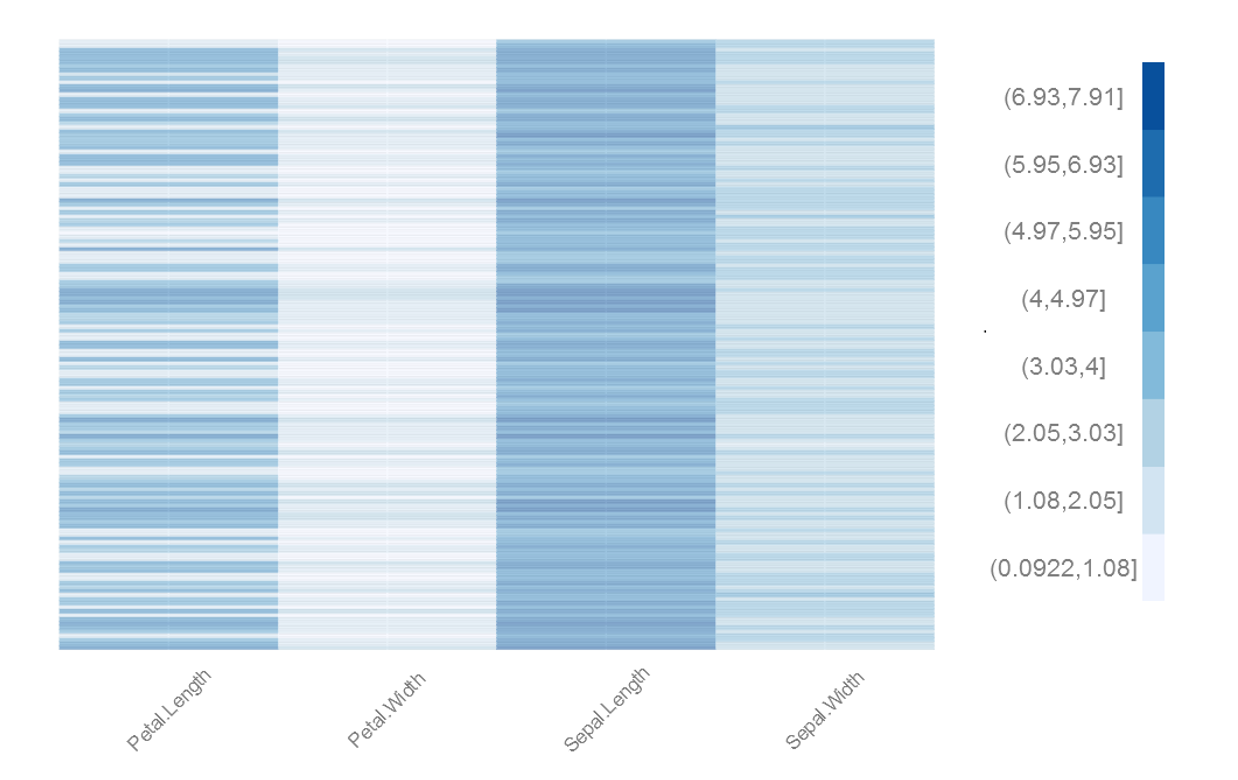
\includegraphics[width=\textwidth,valign=t]{Figures/Iris/HeatmapRawnodendro.png}
		\subcaption{}
		\label{fig:FigHeatmapRawnodendro}
	\end{subfigure}\hfill
	\begin{subfigure}[t]{0.01\textwidth}
		\textbf{b}
	\end{subfigure}
	\begin{subfigure}[t]{0.46\textwidth}
		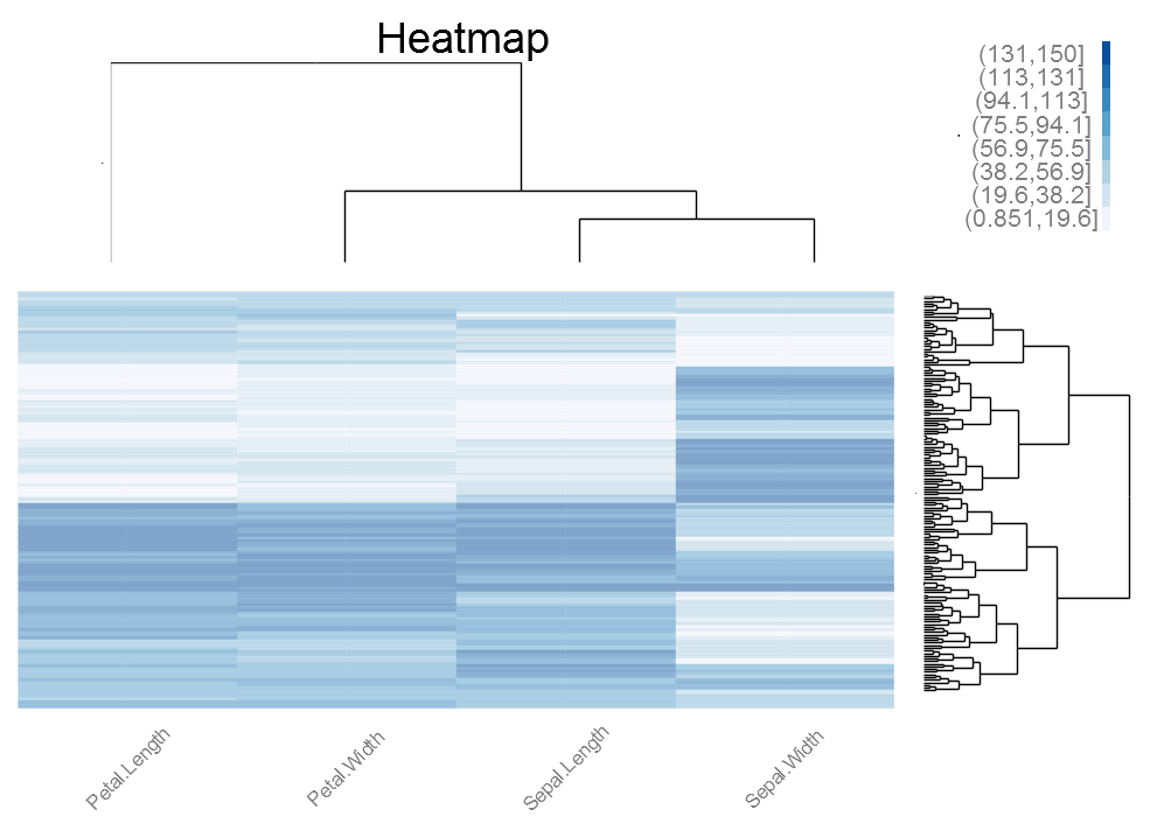
\includegraphics[width=\textwidth,valign=t]{Figures/Iris/HeatmapRanksDendro.png}
		\subcaption{}
		\label{fig:FigHeatmapRanksdendro}
	\end{subfigure}
	\vspace{-1.5\baselineskip}
	\caption{Heatmap of iris dataset for various visualization options. Sample labels are not shown. (a) Heatmap of raw data. Note that there is no evidence for the existence of clusters. (b) Heatmap of data converted to rank with dendrogram and associated row and column sorting. The existence of at least two clusters is clear.}
	\label{fig:FigHeatmap}
\end{figure}

A heatmap provides one of the most minimally-processed ways of visualizing the data, besides simply looking at the data table. However, oftentimes clear trends in the data are obscured on a heatmap because of variations in the range of the data across features. Normalization resolves this issue. The usefulness of heatmaps is further increased by accompanying dendrograms for easy identification of clusters within the data. MX allows users to construct a heatmap of their data and gives them the option to normalize it via conversion to z-scores, quantiles, or ranks. For datasets with less than 100 rows and columns, MX can use hierarchical clustering based on both features and samples to compute two dendrograms for the dataset and display them, reordering the columns and rows as necessary. 

We used the heatmap feature of MX to do our initial exploration of the iris dataset. We found that a simple heatmap of the unnormalized dataset, as shown in Figure~\ref{fig:FigHeatmapRawnodendro}, is not particularly useful. There is no clear structure to the data. This is where normalization schemes, as well as dendrograms and the associated sorting they impose upon the rows and columns of the heatmap, become useful. A heatmap and dendrograms for the ranked data is shown in Figure~\ref{fig:FigHeatmapRanksdendro}. Note that the existence of at least 2 clusters is now apparent.

\subsection{Sample Summary}
\label{subsec:SubSecSample}

\begin{figure}[t!]
	\centering
	\begin{subfigure}[t]{0.01\textwidth}
		\textbf{a}
	\end{subfigure}
	\begin{subfigure}[t]{0.48\textwidth}
		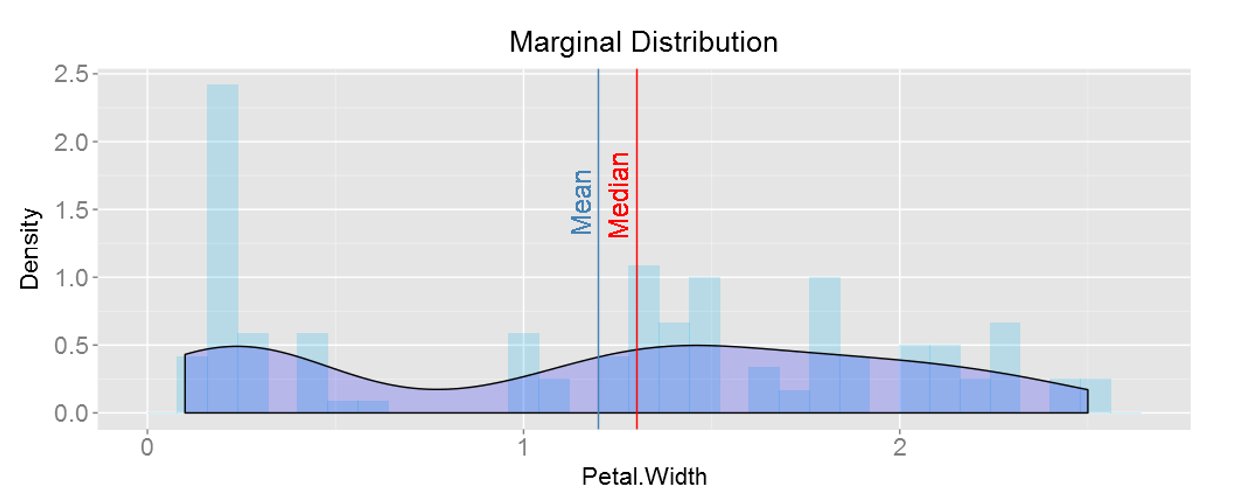
\includegraphics[width=\textwidth,valign=t]{Figures/Iris/MarginalPetalWidthnocond.png}
		\subcaption{}
		\label{fig:FigMarginalNoCond}
	\end{subfigure}\hfill
	\begin{subfigure}[t]{0.01\textwidth}
		\textbf{b}
	\end{subfigure}
	\begin{subfigure}[t]{0.48\textwidth}
		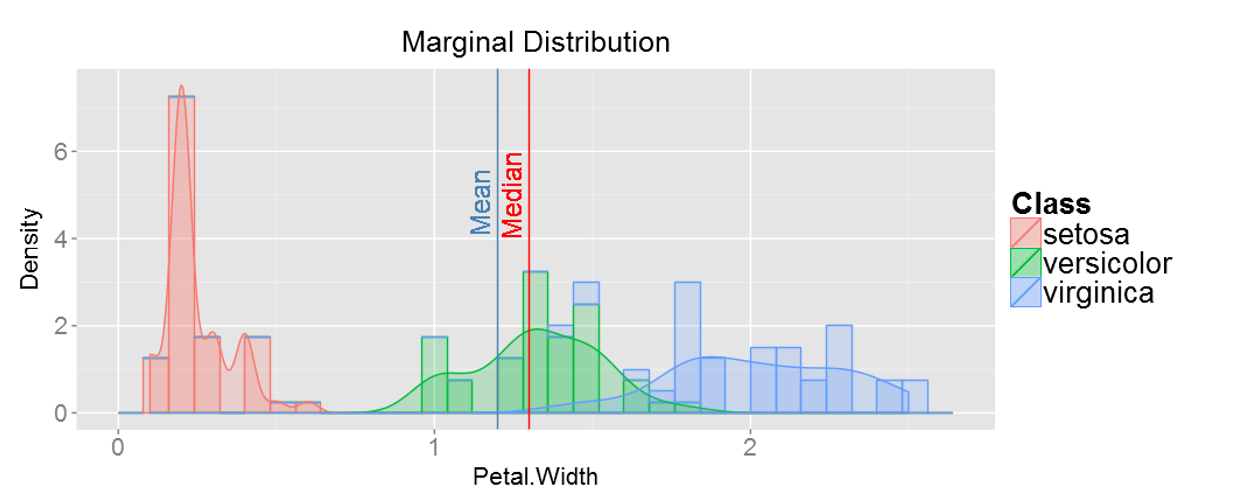
\includegraphics[width=\textwidth,valign=t]{Figures/Iris/MarginalPetalWidth.png}
		\subcaption{}
		\label{fig:FigMarginal}
	\end{subfigure}
	\vspace{-1.5\baselineskip}
	\caption{Marginal of the petal width feature of the iris dataset. (a) Histogram and kernel density estimate of the samples without conditioning on class. Note that it is unclear whether the distribution is multi-modal. (b) Histogram and kernel density estimate of the samples after conditioning on class. It is now clear that the marginal distribution is tri-modal.}
	\label{fig:FigSample}
\end{figure}

One of the initial steps in exploring a new dataset is to look at the marginal distributions of the individual feature columns, as this helps direct future work. MX allows users to visualize these marginal distributions by generating a histogram, a kernel density estimate, or an overlay of both. The mean and median is indicated on the plot. Additionally, if the user labeled a feature as a class label column, he or she has the option of conditioning the marginal on classes. This latter feature is incredibly useful for feature selection and determining the separability of the data based on class labels within the feature space.

We used MX to construct the feature marginals. The distribution for petal width is shown in Figure~\ref{fig:FigMarginalNoCond}. Note that it is unclear whether the distribution is multi-modal and, if it is, how many modes compromise the distribution. This is where conditioning on classes becomes useful (Figure~\ref{fig:FigMarginal}). After conditioning, it is now clear that the marginal is tri-modal and that the petal width feature does a good job of separating the samples into the three classes.

\subsection{Outliers}
\label{subsec:SubSecOutliers}

\begin{figure}[t!]
	\centering
	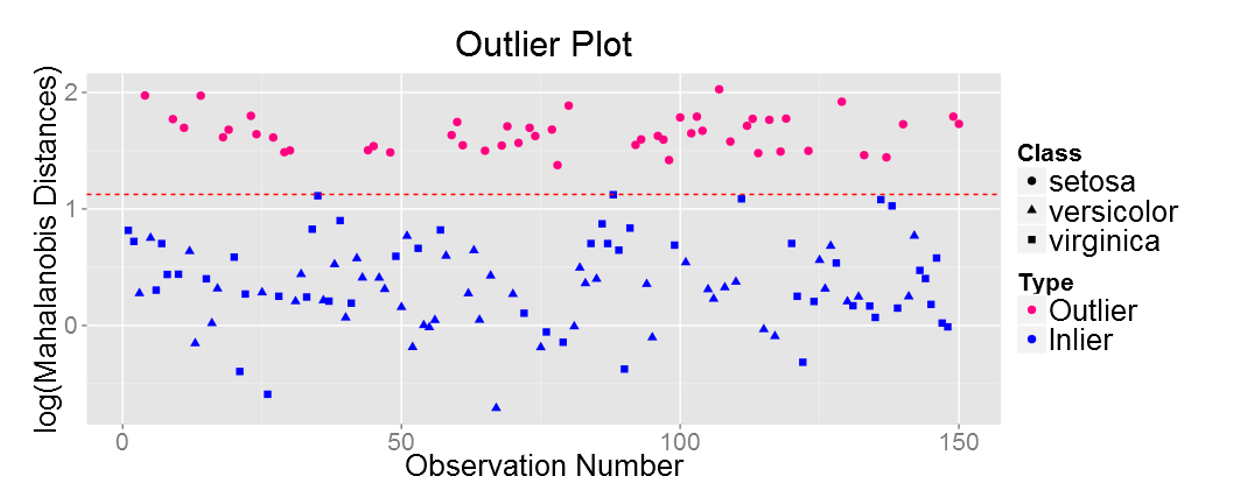
\includegraphics[width=0.95\textwidth]{Figures/Iris/OutliersIris.png}
	\caption{Robust Mahalanobis distances with choice of alpha cut-off value to reject samples as outliers on the iris dataset. Note that 50 of the 150 samples are flagged as outliers.}
	\label{fig:FigOutliers}
\end{figure}

In order to determine outliers it is necessary to determine how far away a specific sample is from other samples by establishing and computing a distance metric. In this case, robust Mahalanobis distances were used, as described in \cite{hubert2008high}. Briefly, a robust estimate of the sample mean and covariance was first approximated via either: 1) the fast minimum covariance determinant algorithm (FAST-MCD), as described in \cite{rousseeuw1999fast}; or 2) the Orthogonalized Gnanadesikan-Kettenring algorithm (OGK), as described in \cite{maronna2002robust}. Since FAST-MCD scales poorly with increasing dimensionality, FAST-MCD was used only for low dimensional datasets, while OGK was used for high dimensional datasets. Next, using these robust measures, the Mahalanobis distance of each sample was computed. As explained by \cite{hardin2012distribution}, the squares of the robust Mahalanobis distances are approximately distributed $\chi^2_n$, where $n$ is the dimensionality of the dataset. It is then possible to define an alpha value above which to reject a sample as an outlier. MX allows the user to set this alpha value and graphically displays the robust Mahalnobis distances and resulting threshold. The robust Mahalanobis distances for the iris data are shown in Figure~\ref{fig:FigOutliers}. Based on the analysis, MX labels 50 of the 150 samples as outliers. This is a very high fraction, and it is quite unlikely that all of these are actually outliers. It is more likely that the samples flagged as outliers actually belong to a single class of iris flower that simply is very far away from the other two classes. When we examined the class labels, this is exactly what we found: all 50 of these samples belong to the \textit{Iris setosa} class, samples from which are, as a whole, apparently quite far from the samples belonging to the \textit{Iris virginica} and \textit{Iris versicolor} classes. Interestingly, the outlier analysis did not indicate a difference in distance between the samples from the \textit{Iris virginica} and \textit{Iris versicolor} classes. 

\subsection{Correlation}
\label{subsec:SubSecCorrelation}

Understanding correlations within a dataset is highly relevant, beyond simply checking assumptions and selecting features to build classifiers. Correlations aid in providing an intuitive understanding of the underlying patterns within the data. For example, in gene expression datasets correlations may indicate the biological importance of various genetic markers (for example, see \cite{shi2012unsupervised}). MX computes the Pearson's correlation amongst features and displays it to the user. To better understand the interactions and distributions of features, MX can also compute the euclidean distance between features. To account for scaling effects, users have the option of pre-processing the data via conversion to z-scores, quantiles, or ranks. Furthermore, users can remove the outliers detected in the outlier tab from the data before computing the metrics. Using these feature on the iris data, we found that all 4 of the features are strongly correlated with one another (data not shown).

\subsection{Feature Summary}
\label{subsec:SubSecFeature}

\begin{figure}[t!]
	\centering
	\begin{subfigure}[t]{0.01\textwidth}
		\textbf{a}
	\end{subfigure}
	\begin{subfigure}[t]{0.48\textwidth}
		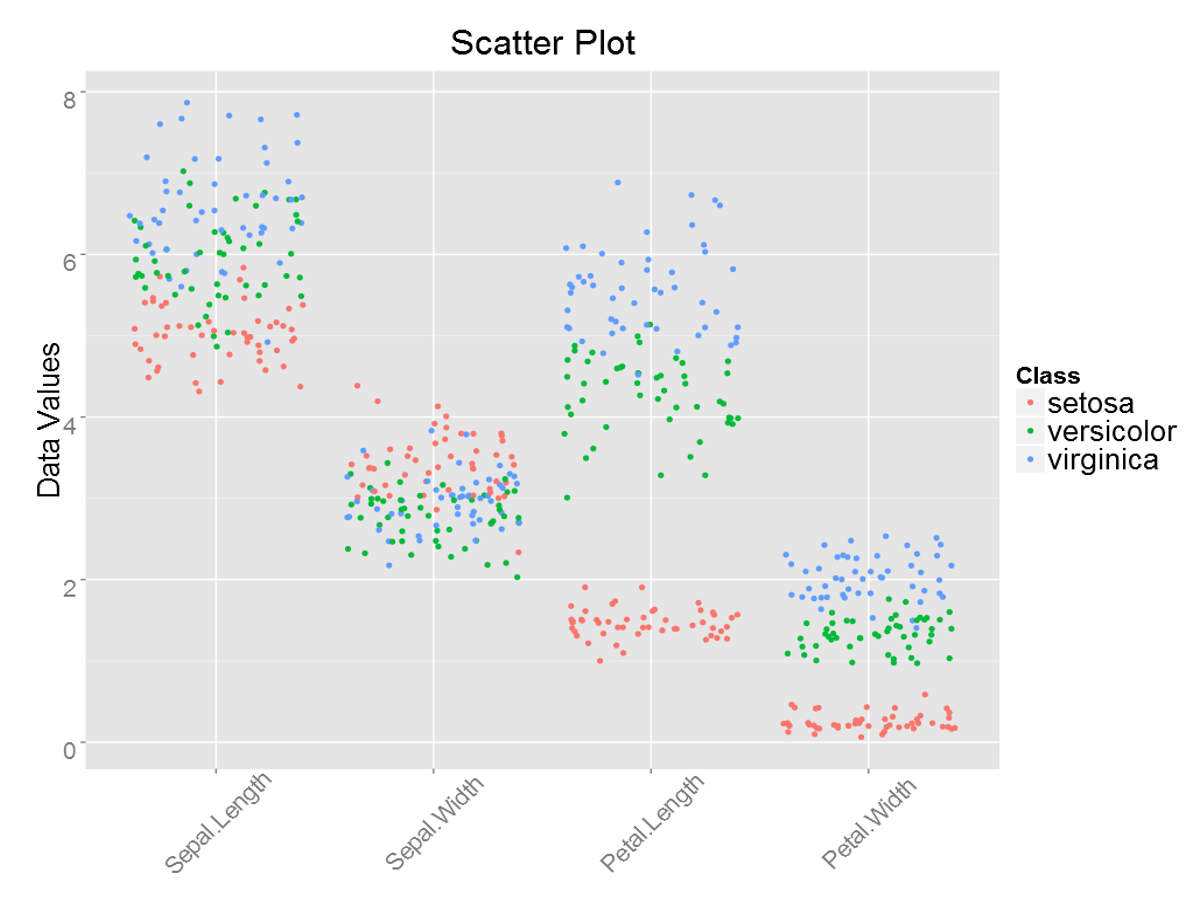
\includegraphics[width=\textwidth,valign=t]{Figures/Iris/ScatterColor.png}
		\subcaption{}
		\label{fig:FigScatter}
	\end{subfigure}\hfill
	\begin{subfigure}[t]{0.01\textwidth}
		\textbf{b}
	\end{subfigure}
	\begin{subfigure}[t]{0.48\textwidth}
		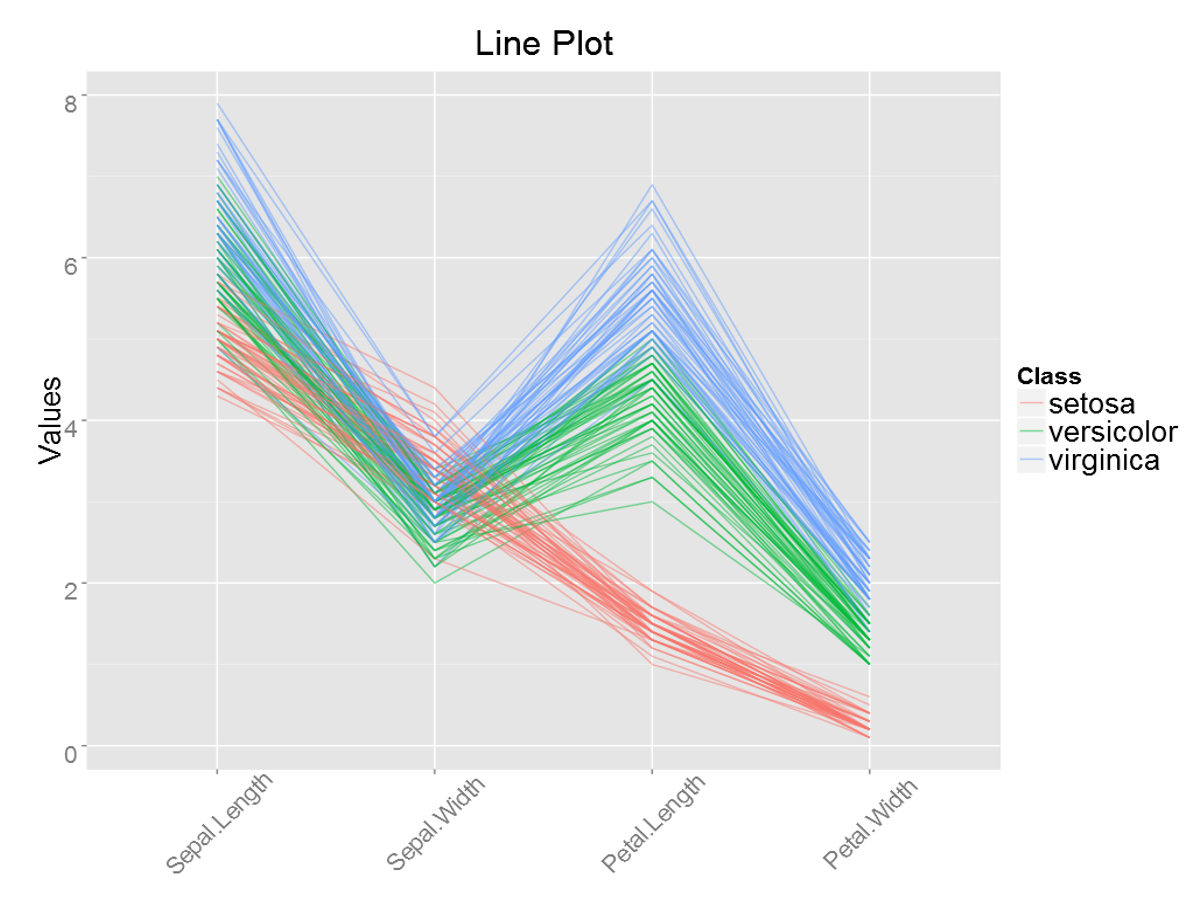
\includegraphics[width=\textwidth,valign=t]{Figures/Iris/LineColor.png}
		\subcaption{}
		\label{fig:FigLine}
	\end{subfigure}
	\vspace{-1.5\baselineskip}
	\caption{Visualization of the samples across all the features in the iris dataset. (a) Jittered scatter plot of the sample values across the features and colored based on class label. Note that the multi-modal nature of the petal width and petal length marginal distributions is clear. It is also apparent that the samples from the \textit{Iris setosa} class are very different from the samples from the other two classes. (b) Line plot showing the behavior of individual samples across the features. Visually, it is clear how differently the samples from the \textit{Iris setosa} class behave compared to samples from the other classes. Note also that we can now visually see the absence of actual outliers.}
	\label{fig:FigFeature}
\end{figure}

MX allows users to visualize the marginal distributions of all the features on the same plot. This is done via a jittered scatter plot, a line plot (where each line represents the values a sample takes on at the corresponding feature), a vector of sample means with standard error bars, a box plot, and a violin plot. In order to ensure that outliers do not skew the visualizations, users have the option of removing outliers detected in the outlier tab from the dataset before generating the plots. 

A jittered scatter plot of the iris data, colored by class label, is shown in Figure~\ref{fig:FigScatter}. The multi-modal nature of the petal length and width features is clear from the plot. Furthermore, the two petal-related features seem to be optimal for separating the data into the three classes. Consistent with the outlier analysis, it is apparent here that the samples from the \textit{Iris setosa} class differ strongly from the samples from the \textit{Iris virginica} and \textit{Iris versicolor} classes. A line plot colored by class label of the same data is shown in Figure~\ref{fig:FigLine}. Again, we see how similar the samples from the \textit{Iris virginica} and \textit{Iris versicolor} classes are to each other and how different they are from the samples from the \textit{Iris setosa} class. Interestingly, we can now visually see that there are no obvious outliers in the data. These observations support the idea that the samples flagged as outliers by MX were not "real" outliers, but instead reflected a distinct class.

\subsection{Embedding \& Clustering}
\label{subsec:SubSecEmbedding}

\begin{figure}[t]
	\centering
	\begin{subfigure}[t]{0.01\textwidth}
		\textbf{a}
	\end{subfigure}
	\begin{subfigure}[t]{0.48\textwidth}
		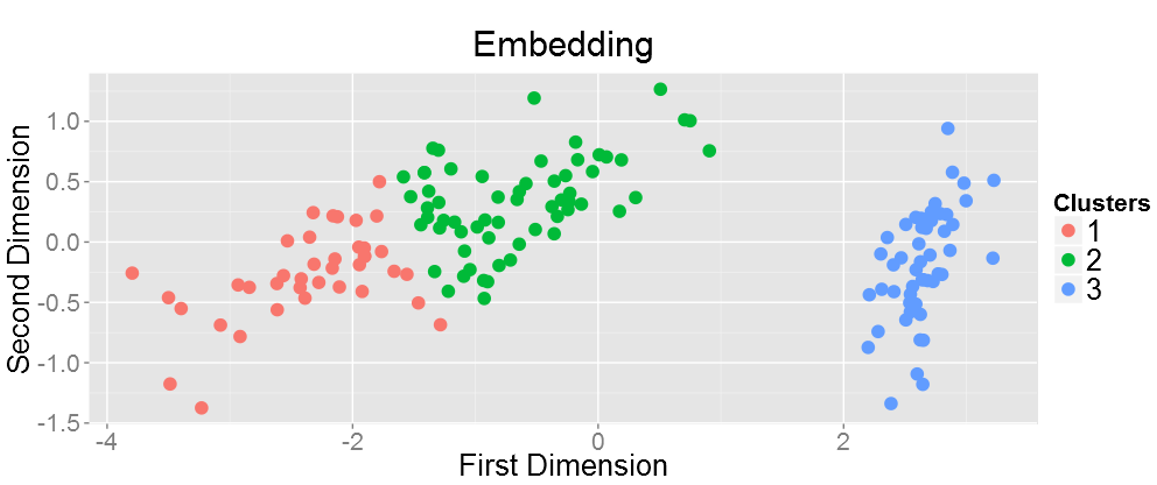
\includegraphics[width=\textwidth,valign=t]{Figures/Iris/EmbedRaw.png}
		\subcaption{}
		\label{fig:FigEmbedRaw}
	\end{subfigure}\hfill
	\begin{subfigure}[t]{0.01\textwidth}
		\textbf{b}
	\end{subfigure}
	\begin{subfigure}[t]{0.48\textwidth}
		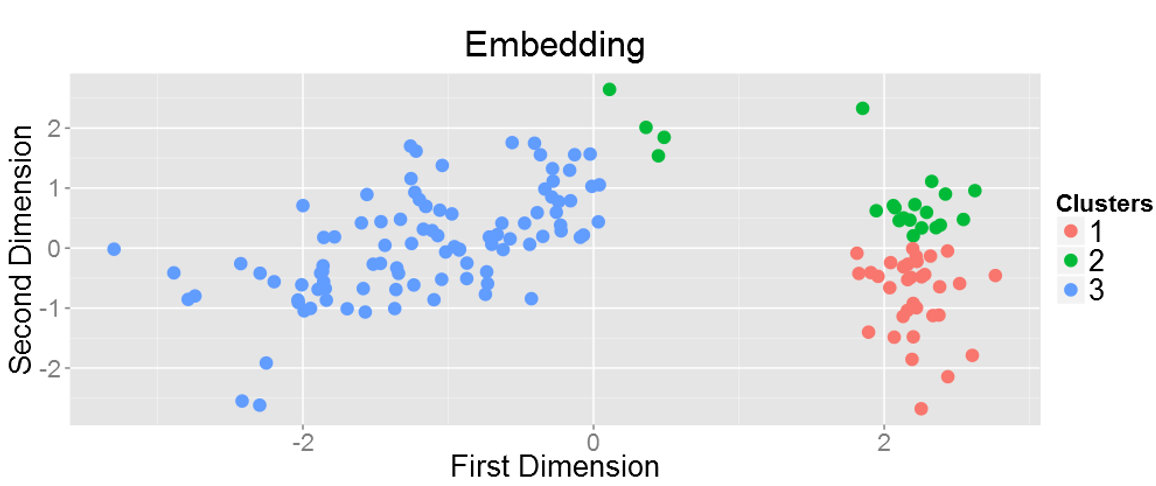
\includegraphics[width=\textwidth,valign=t]{Figures/Iris/EmbedZ.png}
		\subcaption{}
		\label{fig:FigEmbedZ}
	\end{subfigure}
	\vspace{-1.5\baselineskip}
	\caption{Two-dimensional embedding of samples using PCA followed by coloring using labels given by k-means clustering with \textit{k = 3} using (a) raw data and (b) z-score normalized data. Note that the k-means result is significantly worse in (b) compared to (a), to the point that it obfuscates the obvious existence of clear clusters.}
	\label{fig:FigEmbedding}
\end{figure}

One of the most intuitive ways of visualizing bivariate data is a scatter plot. Although this is less straightforward for data with more than two dimensions, various dimensionality reduction techniques can be used to embed the data within a two-dimensional coordinate system for simple examination of general structure and clustering. Dimensionality reduction techniques can be further reduced into linear and non-linear methods, both of which have their own unique advantages and disadvantages (for an overview see \cite{van2009dimensionality}). Within MX we have implemented one linear method -- principle component analysis (PCA) -- and one non-linear method -- t-distributed stochastic neighbor embedding (tSNE). For a thorough description of how tSNE works, see \cite{van2008visualizing}.

PCA is extremely sensitive to: (1) the scaling of the data, and (2) the presence of outliers.  Hence, to overcome (1), MX allows users to normalize the feature columns by converting either to z-scores, quantiles, or ranks. Note that conversion to quantiles or ranks also decreases the sensitivity of the embedding to outliers, hence aiding in overcoming (2). MX also allows users to resolve (2) more directly by giving them the option to remove the outliers detected in the outliers tab before generating the visualization. In order to inform the users of how much information was lost by embedding the data set into two dimensions, MX also displays a scree plot, indicating the percentage of retained variance after PCA. 

For our validation analysis, we implemented two-dimensional embedding via PCA for the raw (Figure~\ref{fig:FigEmbedRaw})  and z-score normalized (Figure~\ref{fig:FigEmbedZ}) iris data after coloring using labels attained via k-means with \textit{k = 3}. Based on these visualizations it is that the k-means clustering result for the z-score normalized data is far worse than the result for the raw data, as it does not indicate the existence of two easily separable clusters. This suggests that the current standard of  normalizing to z-scores is not alway optimal. As we have seen above, the smaller, more distant cluster is likely composed of samples belonging to the \textit{Iris setosa} class.

\section{Conclusion}
\label{sec:conc}

We have created MX, a web application driven by the R Shiny package, that allows for basic data exploration and visualization of small to medium sized datasets. We have included functionality that reflects what we believe to be best practice when exploring a new dataset. We have validated the functionality of MX by demonstrating its capability to characterize the iris flower dataset, including the identification of three distinct classes.

Although the algorithms implemented within MX are relatively simplistic, they are highly relevant to MXs target user base: scientists without the experience necessary to select the statistical techniques to use when initially exploring their data. Indeed, the implemented algorithms give such researchers a foundation from which they can further analyze their data using tools beyond the scope of this work. As such, MX helps resolves a very important issue, that impeded progress in many fields of research. It is a significant step towards supporting all researchers in using appropriate statistical tools to explore their datasets.

%\subsubsection*{Acknowledgments}

%This work is graciously supported by the Defense Advanced Research Projects Agency (DARPA) SIMPLEX program through SPAWAR contract N66001-15-C-4041 and DARPA GRAPHS N66001-14-1-4028. We would also like to thanks Optimize Science for helpful discussions.

\section*{References}
\medskip
\small

\bibliographystyle{Chicago}

\bibliography{BibliographyMX}

\end{document}